%set the master document for easy compilation
%!TEX root = ../D3_5_3.tex

\section{F2.1: Manage\_TrackSideInformation\_Integration}\label{s:F2.1}

\subsection{Component Requirements}

\begin{longtable}{p{.25\textwidth}p{.7\textwidth}}
\toprule
Component name			& Manage\_TrackSideInformation\_Integration \\
\midrule
Link to SCADE model		& {\footnotesize \url{https://github.com/openETCS/modeling/blob/master/model/Scade/System/ObuFunctions/ManageLocationRelatedInformation/BaliseGroup/Manage_TrackSideInformation_Integration/Manage_TrackSideInformation_Integration.etp}} \\
\midrule
SCADE designer			& Bernd Hekele, DB Netz AG \\
\midrule
Description				& The functional block ``Manage\_TrackSideInformation\_Integration'' is responsible for receiving Eurobalise telegrams and Euroradio messages from the API and performs several consistency checks on the inputs.

The block collects the telegrams of balises in order to build balise group messages. Euroradio messages are always delivered as a whole message. On each message, a consistency check is performed, before the data is validated according to the driving direction of the train. In general, messages not designated for the current driving direction of the train are not forwarded for further processing. After applying consistency checks, the data direction is validated. Finally, the received message is handled in the InformationFilter subcomponent. The InformationFilter may, depending on level, mode and announced level transitions and radio handover scenarios, let information pass immediately, reject information, or buffer information for some cycles until certain conditions apply and the information will be passed. Information in this sense is packets in the context of messages.\\
\midrule
Input documents			& See subcomponents.\\
\midrule
Safety integrity level	& 4 \\
\midrule
Time constraints		& The component has to be able to receive balise telegrams and radio messages according to the ETCS performance requirements, c.f. \cite{subset-41}. In highspeed traffic, a group of 8 balises must be read in about 250 msec. In addition, 1 message per sec. on the radio interface is to be expected.\\
\midrule
API requirements 		& Interfaces to this unit are defined in the API sections [BTM], [EURORADIO], [ODO]. In these sections, also a detailed definition of the concepts implemented on those interfaces is documented.
\todo[inline]{reference sections correctly once these are completed}  \\
\bottomrule
\end{longtable}


\subsection{Interface}

An overview of the interface of component Manage\_TrackSideInformation\_Integration is shown in Figure~\ref{f:receiveAndCheckConsistencyArch}. The inputs and outputs are described in detail in Section~\ref{s:Manage_Trackside_inputs} respectively \ref{s:Manage_Trackside_outputs}. Subcomponents are described in Section~\ref{s:receivetrackdata_subcomponents}.

\begin{figure}[H]
\center
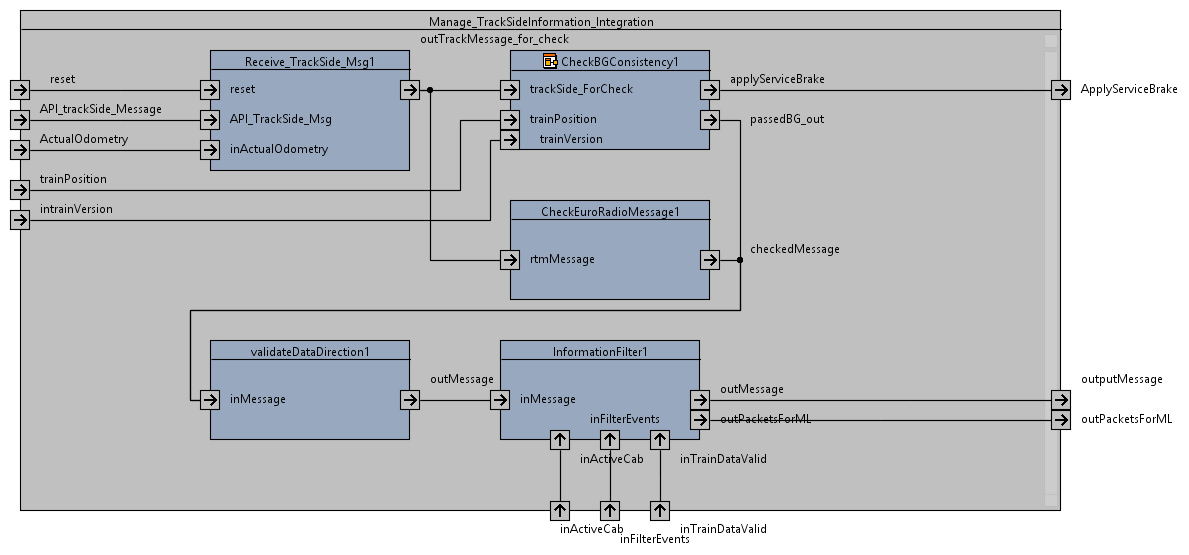
\includegraphics[width=\textwidth]{./images/Figure_1_IBD_Manage_TrackSideInformation_Integration_1.png}
\caption{Manage\_TrackSideInformation\_Integration component SysML diagram.}\label{f:receiveAndCheckConsistencyArch}
\end{figure}


\subsubsection{Inputs}\label{s:Manage_Trackside_inputs}

\paragraph{fullChecks}

\begin{longtable}{p{.25\textwidth}p{.7\textwidth}}
\toprule
Input name				& fullChecks \\
\midrule
Description				& Indicates, if all checks on the message should be performed. This parameter is for testing purposes only and has to be replaced by a constant in real operation.\\
\midrule
Source					& This item is only relevant in verification phases. In a real system checks are always activated. \\ 
\midrule
Type					& bool \\
\midrule
Valid range of values	& 
\begin{description}
\item[true] All checks are performed.
\item[false] Component InformationFilter is deactivated.
\end{description} \\
\midrule
Behaviour when value is at boundary	& n/a \\
\midrule
Behaviour for values out of valid range	& n/a \\
\midrule
Behaviour when value is erroneous, absent or unwanted (i.e. spurious) & n/a\\
\bottomrule
\end{longtable}


\paragraph{API\_trackSide\_Message}

\begin{longtable}{p{.25\textwidth}p{.7\textwidth}}
\toprule
Input name				& API\_trackSide\_Message \\
\midrule
Description				& Track side message received from the API. The API performs preprocessing of RTM and BTM messages and delivers a maximum of a single message per cycle. The structure of this message is defined in the API [BTM] and [EURORADIO] sections. The input consists of the following main components:\\
&
\begin{description}
\item[valid](bool) Indicates the information has been refreshed in the cycle.
\begin{description}
\item[true]: Information is updated in this cycle.
\item[false]: Information is unchanged.
\end{description}
\end{description}\\
&
\begin{description}
\item[systemTimeMsgReceived](Obu\_BasicTypes\_Pkg::T\_internal\_Type): Timestamp when the system (i.e. the train) has received the message. The parameter is set either by RTM or by BTM modules.
\end{description}\\
&
\begin{description}
\item[msg\_type](Common\_Types\_Pkg::MsgSource\_T) source of this information. 
\begin{description}
\item[msrc\_undefined] indicates the information is not defined. This input is expected when valid flag is false.
\item[msrc\_Euroradio] indicates the information is a euroradio message.
\item[msrc\_Eurobalise] indicates the information is a balise telegram.
\end{description}
Other values of this enumeration are not expected in this model.
\end{description}\\
&
\begin{description}
\item[btm\_msg](API\_Msg\_Pkg::API\_TelegramHeader\_T) Telegram header with some additional information provided by the btm-module. The header is structured as follows:
\begin{description}
\item[present](bool) Telegram information has been received via btm and the information of this telegram is present. 
\item[checkResult](bool) The telegram is checked after reception at the btm. Typical checks are checksum-tests or checks at conversion of the types from bit-layout to the presentation in the evc. If checkResult is false the information may not be used. The information is evaluated in the checkBGConsistency component of this model.
\item[api\_bad\_balise\_received](bool) The telegram reception was disturbed. Again, the information related to this telegram may not be used in the EVC.
\item[api\_header](API\_Msg\_Pkg::API\_TelegramHeader\_T) Header of the telegram similar to subset 26 section 8.4.2.1. The information in the telegram is not packed on bit-boundaries.
\item[centerOfBalisePosition](BG\_Types\_Pkg::centerOfBalisePosition\_T) Location of the balise as determined by the antenna of the train. The information is extended with inaccuracies of the measurement given by the BTM.
\end{description}
\end{description}\\
&
\begin{description}
\item[rtm\_msg](API\_Msg\_Pkg::API\_RadioMsgHeader\_T) Radio message header with some additional information added by the RTM module. The information is structured as follows:
\begin{description}
\item[present](bool) Radio message has been received via rtm and the information of this message is present. 
\item[apiConsistencyError](bool) The message is checked after reception at the btm. Typical checks are checksum-tests or checks at conversion of the types from bit-layout to the presentation in the evc. If apiConsistencyError is false the information may not be used. The information is evaluated in the checkRadioMessage component of this model.
\item[Radio\_Common\_Header](Radio\_Types\_Pkg::\newline Radio\_TrackTrain\_Header\_T) Header of the radio-message as defined in subset 26 section 8.4.4.6.1. In the SRS, depending on the concrete message, some optional variables are defined. In our implementation all optional variables are foreseen. In order to indicate the availability of variables the component radioMetadata is used (see below).
\item[radioMetadata](Common\_Types\_Pkg::RadioMetadata\_T) Metadata for optional variables in the common radio message header. For each optional component a presence indicator of type bool is in the list.  
\item[sendingRBC\_Id](Common\_Types\_Pkg::RBC\_Id\_T) Identifies the RBC as it is known at the RTM. Information is added to the interface in the RTM.
\begin{description}
\item[packets](Common\_Types\_Pkg::CompressedPackets\_T) Packets as received as a part of the telegram or radio message. The structure is set-up and can be accessed by library routines of the trackMessages component of the system. In the manage\_trackside\_Messages component packets may be changed to being absent (e.g., by the function validateDataDirection or by the InformationFilter.). If packets have to be treated only this valid indicator is changed. No other parts of the packets are accessed.
\end{description}
\end{description}
\end{description}
\\
\midrule
Source					& API\_fromTrack 
\\ 
\midrule
Type					& API\_Msg\_Pkg::API\_TrackSideInput\_T \\
\midrule
Valid range of values	& Access to the information has to be guarded by the valid flag and similar flags deeper in the structure of the interface. Checks on individual values of message components, telegrams and packets are part of the decoding function. We assume information to be valid in this part of the system.\\
\midrule
Behaviour when value is at boundary	& n/a (structure)\\
\midrule
Behaviour for values out of valid range	& n/a\\
\midrule
Behaviour when value is erroneous, absent or unwanted (i.e. spurious) &n/a\\
\bottomrule
\end{longtable}


\paragraph{ActualOdometry}

\begin{longtable}{p{.25\textwidth}p{.7\textwidth}}
\toprule
Input name				& ActualOdometry \\
\midrule
Description				& Odometry data provided by the external odometry module of the train. It contains relative location information with inaccuracies. In this model only information related to the position of the train is used (odo-component). A valid flag of the odometer input indicates the hardware is working and the parameter may be used.\\
\midrule
Source					& API\_Odometery \\ 
\midrule
Type					& Obu\_BasicTypes\_Pkg::odometry\_T \\
\midrule
Valid range of values	& From the ODO component the nominal position is used. No plausibility checks on the component are done. Any integer value is allowed. \\
\midrule
Behaviour when value is at boundary	& Boundary value may lead to jump of the calculation in negative ranges. As a result the train may not being able to complete the reading of a balise group. In consequence, this results in a balise group error and in a service brake reaction of the train.\\
\midrule
Behaviour for values out of valid range	& Same as description at boundary.\\
\midrule
Behaviour when value is erroneous, absent or unwanted (i.e. spurious) & Same as description at boundary.\\

\bottomrule
\end{longtable}

\paragraph{reset}

\begin{longtable}{p{.25\textwidth}p{.7\textwidth}}
\toprule
Input name				& reset \\
\midrule
Description				& The reset input is used to delete all data stored in the module (e.g.~collected balise telegrams, which do not yet form a complete message). If the input is set to true, all data kept in the module is deleted and no input is accepted. The reset option is to be used when the EVC is started or in system error scenarios.\\
\midrule
Source					& function not yet defined
\\ \midrule
Type					& bool \\
\midrule
Valid range of values	& 
\begin{description}
\item[true] All data kept in the module is deleted and no input is accepted.
\item[false] No action. Data at input is accepted.
\end{description} \\
\midrule
Behaviour when value is at boundary	& n/a\\
\midrule
Behaviour for values out of valid range	& n/a\\
\midrule
Behaviour when value is erroneous, absent or unwanted (i.e. spurious) & n/a\\
\bottomrule
\end{longtable}
\newpage
\paragraph{trainPosition}

\begin{longtable}{p{.25\textwidth}p{.7\textwidth}}
\toprule
Input name				& trainPosition \\
\midrule
Description				& Contains the current position of the train. This input is used for validation of the direction of packets and for checks of balise groups. Most important information in this input is the LRBG and the prevLRBG component. This identifies the last two balise group passed by the train.\\
\midrule
Source					& CalculateTrainPosition \\ 
\midrule
Type					& TrainPosition\_Types\_Pck::trainPosition\_T \\
\midrule
Valid range of values	& A valid flag is used in this input to indicate data is provided correctly.\\
\midrule
Behaviour when value is at boundary	& n/a\\
\midrule
Behaviour for values out of valid range	& n/a\\
\midrule
Behaviour when value is erroneous, absent or unwanted (i.e. spurious) & n/a\\
\bottomrule
\end{longtable}

\paragraph{modeAndLevel}

\begin{longtable}{p{.25\textwidth}p{.7\textwidth}}
\toprule
Input name				& modeAndLevel \\
\midrule
Description				& Provides the current level and mode of the EVC. Mode and Level are used by the InformationFilter subcomponent.\\
\midrule
Source					& ModeAndLevel \\ 
\midrule
Type					& BG\_Types\_Pkg::ModeAndLevelStatus\_T \\
\midrule
Valid range of values	& n/a\\
\midrule
Behaviour when value is at boundary	& n/a\\
\midrule
Behaviour for values out of valid range	& n/a\\
\midrule
Behaviour when value is erroneous, absent or unwanted (i.e. spurious) & n/a\\
\bottomrule
\end{longtable}


\paragraph{tNvContact}

\begin{longtable}{p{.25\textwidth}p{.7\textwidth}}
\toprule
Input name				& tNvContact \\
\midrule
Description				& For monitoring the safe radio connection, this national value is needed as an input. This parameter is used in the radioCheck component of this model. \\
\midrule
Source					& Radio Management\\ 
\midrule
Type					& Obu\_BasicTypes\_Pkg::T\_internal\_Type \\
\midrule
Valid range of values	& Positive integer. \\
\midrule
Behaviour when value is at boundary	& When boundary is reached the input will jump to 0.\\
\midrule
Behaviour for values out of valid range	& if negative this parameter will result in a radio message sequence error. Connection to the rbc will be closed.\\
\midrule
Behaviour when value is erroneous, absent or unwanted (i.e. spurious) & See above.\\
\bottomrule
\end{longtable}

\paragraph{intrainVersion}

\begin{longtable}{p{.25\textwidth}p{.7\textwidth}}
\toprule
Input name				& M\_VERSION \\
\midrule
Description				& For monitoring the safe radio connection, this national value is needed as an input. This parameter is used in the radioCheck component of this model. \\
\midrule
Source					& EVC Configuration
\todo[inline]{Proposal: Function not yet visible in the document. Implemented in the evc main model.}\\ 
\midrule
Type					& M\_VERSION \\
\midrule
Valid range of values	& Enumerated values.\\
\midrule
Behaviour when value is at boundary	& Value check will reject radio message resp. balise telegram. In the consequence train will stop resp. session rejected. \\
\midrule
Behaviour for values out of valid range	& Value check will reject radio message resp. balise telegram. In the consequence train will stop resp. session rejected.\\
\midrule
Behaviour when value is erroneous, absent or unwanted (i.e. spurious) & See above. \\
\bottomrule
\end{longtable}


\paragraph{lastRelevantEventTimestamp}

\begin{longtable}{p{.25\textwidth}p{.7\textwidth}}
\toprule
Input name				& lastRelevantEventTimestamp \\
\midrule
Description				& For monitoring the safe radio connection, it is necessary that the time between two packets is less than the value of {T\_NVCONTACT}.\newline
In situations like level changes or announced radio holes, not the timestamp of the last message is relevant for comparison, but the timestamp of the last relevant event. This can for example be the timestamp of the level change or the timestamp of the moment, when the train was passing the end of the radiohole.

For performing this check, the timestamp of the last relevant event is provided to the model as an {T\_internal\_Type}-type. \\
\midrule
Source					& collectRadioMessages
\todo[inline]{Proposal: Function not yet visible in the document. Implemented in the evc main model. Covers functions distributed in the evc model}\\ 
\midrule
Type					& Obu\_BasicTypes\_Pkg::T\_internal\_Type \\
\midrule
Valid range of values	& Positive integer.\\
\midrule
Behaviour when value is at boundary	& Value will jump to 0. This may result in calculations of durations with negative result. As a consequence, the train will react with the loss of the communication session.\\
\midrule
Behaviour for values out of valid range	& See above.\\
\midrule
Behaviour when value is erroneous, absent or unwanted (i.e. spurious) & See above.\\
\bottomrule
\end{longtable}


\paragraph{connectionStatus}

\begin{longtable}{p{.25\textwidth}p{.7\textwidth}}
\toprule
Input name				& connectionStatus \\
\midrule
Description				& Status information about the radio connection. The information is needed to perform the timing check, which depends on the connection state in the radioCheck component. \\
\midrule
Source					& ManageRadioCommunication \\ 
\midrule
Type					& Radio\_Types\_Pkg::sessionStatus\_Type \\
\midrule
Valid range of values	& 
\begin{description}
\item[DISCONNECTED] The OBU is currently not connected to a RBC.
\item[CONNECTING] The OBU is currently connecting to the RBC. Received messages belong to the process of establishing a connection.
\item[CONNECTION\_ESTABLISHED] The connection to the RBC is established.
\end{description} \\
\midrule
Behaviour when value is at boundary	& n/a\\
\midrule
Behaviour for values out of valid range	& n/a\\
\midrule
Behaviour when value is erroneous, absent or unwanted (i.e. spurious) & n/a\\
\bottomrule
\end{longtable}


\paragraph{inSupervisingRbcId}

\begin{longtable}{p{.25\textwidth}p{.7\textwidth}}
\toprule
Input name				& inSupervisingRbcId \\
\midrule
Description				& For the InformationFilter subcomponent, the information which radio messages are sent by the supervising RBC is needed. To recognize these messages, the identifier of the supervising RBC is needed. \\
\midrule
Source					& ManageRadioCommunication\\ 
\midrule
Type					& int \\
\midrule
Valid range of values	& 0, 1, 2
 \\
\midrule
Behaviour when value is at boundary	& n/a\\
\midrule
Behaviour for values out of valid range	&  Is interpreted as no valid radio connection.\\
\midrule
Behaviour when value is erroneous, absent or unwanted (i.e. spurious) & Is interpreted as no valid radio connection.\\
\bottomrule
\end{longtable}


\paragraph{inAnnouncedBGs}

\begin{longtable}{p{.25\textwidth}p{.7\textwidth}}
\toprule
Input name				& inAnnouncedBGs \\
\midrule
Description				& Provides information about balise groups as known in the EVC. This information is generated by the CalculateTrainPosition component based on the linking information received from track side and on the balise groups passed by the train.\\
\midrule
Source					& CalculateTrainPosition \\ 
\midrule
Type					& TrainPosition\_Types\_Pck::positionedBGs\_T \\
\midrule
Valid range of values	& Each balise group netry is identified by an valid flag. \\
\midrule
Behaviour when value is at boundary	& n/a\\
\midrule
Behaviour for values out of valid range	& n/a\\
\midrule
Behaviour when value is erroneous, absent or unwanted (i.e. spurious) & n/a\\
\bottomrule
\end{longtable}


\paragraph{q\_nvlocacc}

\begin{longtable}{p{.25\textwidth}p{.7\textwidth}}
\toprule
Input name				& q\_nvlocacc \\
\midrule
Description				& This national value determines the location accuracy. Needed as input for checkBGConsistency.  \\
\midrule
Source					& trackAtlas\\ 
\midrule
Type					& Q\_NVLOCACC \\
\midrule
Valid range of values	& 0 \ldots 63\\
\midrule
Behaviour when value is at boundary	& No impact.\\
\midrule
Behaviour for values out of valid range	& Will result in wrong calculation of inaccuracy of the train.\\
\midrule
Behaviour when value is erroneous, absent or unwanted (i.e. spurious) & See above.\\
\bottomrule
\end{longtable}


\paragraph{inActiveCab}

\begin{longtable}{p{.25\textwidth}p{.7\textwidth}}
\toprule
Input name				& inActiveCab \\
\midrule
Description				& Indicates the cab is active. Used by InformationFilter. \\
\midrule
Source					& TIU\\ 
\midrule
Type					& bool\\
\midrule
Valid range of values	& true, false\\
\midrule
Behaviour when value is at boundary	& n/a\\
\midrule
Behaviour for values out of valid range	& n/a\\
\midrule
Behaviour when value is erroneous, absent or unwanted (i.e. spurious) & n/a\\
\bottomrule
\end{longtable}

\paragraph{inTrainDataValid}

\begin{longtable}{p{.25\textwidth}p{.7\textwidth}}
\toprule
Input name				& inTrainDataValid \\
\midrule
Description				& Indicates train data have been validated by the RBC. Used by InformationFilter. \\
\midrule
Source					& trainData\\ 
\midrule
Type					& bool\\
\midrule
Valid range of values	& true, false\\
\midrule
Behaviour when value is at boundary	& n/a\\
\midrule
Behaviour for values out of valid range	& n/a\\
\midrule
Behaviour when value is erroneous, absent or unwanted (i.e. spurious) & n/a\\
\bottomrule
\end{longtable}

\paragraph{inFilterEvents}

\begin{longtable}{p{.25\textwidth}p{.7\textwidth}}
\toprule
Input name				& inFilterEvents \\
\midrule
Description				& A set of events needed for controlling the InformationFilter. For details see valid range of values row in this table.\\
\midrule
Source					& ModeAndLevels, MoRC
\\  
\midrule
Type					& Common\_Types\_Pkg::filterRelatedEvents\_T\\
\midrule
Valid range of values	& This input is a complex structure consisting out of the following components:
\begin{description}
\item[pendingL1Transition](bool) Indicates if an announced LEVEL 1 transition is present. Used for Level filter exception [1]. The information is indicating the status.
Note: this indication can be evaluated based on information available in the InformationFilter. The input is not used from outside the main component Manage\_TrackSide\_Information.
\item[pendingL2L3Transition](bool) Indicates if an announced LEVEL 2 or Level 3 transition is present. Used for Level Filter exception [2]. The information is indicating the status.
Note: this indication can be evaluated based on information available in the InformationFilter. The input is not used from outside the main component Manage\_TrackSide\_Information.
\item[pendingAckOfTrainDataFromRBC](bool) Indicates if the acknowledgement of train data is pending. Used for Level filter exception [3].
\item[emergencyStopAccepted](bool): Indicate if the train performs an emergency brake. Used for Level filter exception [5].
\item[lastAckTextMessageId](int) The ID of the last acknowledged text message ID. Used for Level filter exception [12]. The SRS requires text messages to restrict from double sending to the DMI when handled in the filter. This function is currently not implemented. 
\item[pendingNTCTransition](bool) Indication if an announced LEVEL NTC transition is present. Used for Level filter exception [6,7].
\item[SPPAndGradientOnBoard](bool) Speed Profile and Gradient Profile received and available on board. This information may be part of the actual incoming message.
\item[MACoverNotFullLength](bool) MA does not cover full length of the trip. Information from trackAtlas.
\end{description}\\
\midrule
Behaviour when value is at boundary	& n/a\\
\midrule
Behaviour for values out of valid range	& n/a\\
\midrule
Behaviour when value is erroneous, absent or unwanted (i.e. spurious) & n/a\\
\bottomrule
\end{longtable}

\paragraph{transitionPositionPassed}

\begin{longtable}{p{.25\textwidth}p{.7\textwidth}}
\toprule
Input name				& transitionPositionPassed \\
\midrule
Description				& The position of the requested level transition has been passed. This information is used by InformationFilter subcomponent to clean data after level management reactions.
\\
\midrule
Source					& ModeAndLevels\\ 
\midrule
Type					&bool\\
\midrule
Valid range of values	& true, false\\
\midrule
Behaviour when value is at boundary	& n/a\\
\midrule
Behaviour for values out of valid range	& n/a\\
\midrule
Behaviour when value is erroneous, absent or unwanted (i.e. spurious) & n/a\\
\bottomrule
\end{longtable}
\subsubsection{Outputs}\label{s:Manage_Trackside_outputs}

\paragraph{outputMessage}

\begin{longtable}{p{.25\textwidth}p{.7\textwidth}}
\toprule
Output name				& outputMessage \\
\midrule
Description				& Combines both balise and radio messages to one common datatype. This datatype contains all variables and packets, which are possible for the given scenario. In each cycle at most one valid message is put to the output. The InformationFilter might take the last processed one or a message from stack - depending on the information stored and on the status of the evc. The component consists of the following building blocks:\\
&
\begin{description}
\item[valid] Information about the status of this message.
\begin{description}
\item[true] The information is valid, a new message is now visible at the output. The valid flag (and the message as such) will only be present for one cycle.
\item[false] No valid message is available.
\end{description}
\end{description}\\
&
\begin{description}
\item[source](Common\_Types\_Pkg::MsgSource\_T) Source of this information. 
\begin{description}
\item[msrc\_undefined] Indicates the information is not defined. This input is expected when valid flag is false.
\item[msrc\_Euroradio] Indicates the information is a euroradio message.
\item[msrc\_Eurobalise] Indicates the information is a balise telegram.
\end{description}
Other values of this enumeration are not expected in this model.
\item[radioMetadata](Common\_Types\_Pkg::RadioMetadata\_T) Metadata for optional variables in the common radio message header. For each optional component a presence indicator of type bool is in the list.  
\item[BG\_Common\_Header](BG\_Types\_Pkg::BG\_Header\_T) Balise group message header with some additional information. This header collects information from the balise telegram headers together with the location and orientation of the balise group related to the driving direction.

\item[Radio\_Common\_Header](Radio\_Types\_Pkg::\newline Radio\_TrackTrain\_Header\_T) Radio message header with some additional information added by the RTM module. Variables of messages which are not present in all messages are available in the header, but controlled by the radio metadata.
\item[packets](Common\_Types\_Pkg::CompressedPackets\_T) Packets as received as a part of the telegram or radio message. The structure is set-up and can be accessed by library routines of the trackMessages component of the system. In the manage\_trackside\_Messages component packets my be changed to being absent (e.g., by the function validateDataDirection or by the InformationFilter.). If packets have to be treated only this valid indicator is changed. No other parts of the packets are changed.
\end{description}
\\
\midrule
Destination				& (nearly) all functions
\todo[inline]{Proposal: This is not reasonable in all cases. This output is similasr to Lib functions.}\\ 
\midrule
Type					& Common\_Types\_Pkg::ReceivedMessage\_T \\
\midrule
Valid range of values	& n/a\\
\midrule
Behaviour when value is at boundary	& n/a\\
\midrule
Behaviour for values out of valid range	& n/a\\
\midrule
Behaviour when value is erroneous, absent or unwanted (i.e. spurious) & n/a\\
\bottomrule
\end{longtable}


\paragraph{ApplyServiceBrake}

\begin{longtable}{p{.25\textwidth}p{.7\textwidth}}
\toprule
Output name				& ApplyServiceBrake \\
\midrule
Description				&  Indicates if the balise group the train just passed could not be processed correctly. The check results in the request for a service break. \\
\midrule
Destination				& SpeedSupervision\_Integration\\ 
\midrule
Type					& bool \\
\midrule
Valid range of values	& true, false\\
\midrule
Behaviour when value is at boundary	& n/a\\
\midrule
Behaviour for values out of valid range	& n/a\\
\midrule
Behaviour when value is erroneous, absent or unwanted (i.e. spurious) & n/a\\
\bottomrule
\end{longtable}


\paragraph{BadBaliseMessageToDMI}

\begin{longtable}{p{.25\textwidth}p{.7\textwidth}}
\toprule
Output name				& BadBaliseMessageToDMI \\
\midrule
Description				& Information to be passed to the DMI to indicate the reception of a ``bad balise'' to the driver. \\
\midrule
Destination				& manage\_DMI\_Output\_Pkg
\\
\midrule
Type					& bool \\
\midrule
Valid range of values	& true, false\\
\midrule
Behaviour when value is at boundary	& n/a\\
\midrule
Behaviour for values out of valid range	&  n/a\\
\midrule
Behaviour when value is erroneous, absent or unwanted (i.e. spurious) &  n/a\\
\bottomrule
\end{longtable}


\paragraph{outCheckErrors}

\begin{longtable}{p{.25\textwidth}p{.7\textwidth}}
\toprule
Output name				& outCheckErrors \\
\midrule
Description				& Error flags for errors reported at the check procedures at messages. For details see valid range of values row of this table.\\
\midrule
Destination				& JRU
\todo[inline]{Proposal: Use input name of F2 or the exact SCADE component name here for consitency and traceablity. This error Information is actually soemthing which is needed for tracebaility in testing and for the JRU}\\ 
\midrule
Type					& Common\_Types\_Pkg::MSG\_Errors\_T\\
\midrule
Valid range of values	& This output is a complex structure mainly consisting out of boolean values. The boolean variables are set true if an error in the particular parameter has been detected and false otherwise.
\begin{description}
\item[linkedBGError](bool) Reported by checkBGConsistency. Error in a linked BGH - Message has been detected.
\item[unlinkedBGError](bool) Reported by checkBGConsistency. Error in an unlinked BGH - Message has been detected.
\item[BG\_versionIncompatible](bool) Reported by checkBGConsistency. Version of received Balises is not compliant with the train. Balises cannot be used.
\item[radioSequenceError](bool) Reported by checkEuroRadioMessage. The sequence of messages in the input channel is not correct. This check is based in t\_train of the incoming radio messages.
\item[tNvContactError](bool) Reported by checkEuroRadioMessage. The time for receiving the next radio message has been exceeded. This indicates lost radio messages.
\item[otherTimingError](bool) Reported by checkEuroRadioMessage. Other timing errors.
\item[radioMessageConsistencyError](bool) Reported by checkEuroRadioMessage. Inconsistencies in the contents of radio messages have been detected.
\item[nid\_c](NID\_C) Reported by checkBGConsistency. If known id of the erroneous balise group.
\item[nid\_errorbg](NID\_ERRORBG) Reported by checkBGConsistency. If known id of the erroneous balise group.
\end{description}
\\
\midrule
Behaviour when value is at boundary	& n/a\\
\midrule
Behaviour for values out of valid range	& n/a\\
\midrule
Behaviour when value is erroneous, absent or unwanted (i.e. spurious) & n/a\\
\bottomrule
\end{longtable}


\paragraph{forLevelManagement}

\begin{longtable}{p{.25\textwidth}p{.7\textwidth}}
\toprule
Output name				& errorUnlinkedBG \\
\midrule
Description				& The InformationFilter component has to provide information to the EVC components according to the actual level and radio state. In order to trigger the level change level management needs to know about avaialblity of track profiles and other components in order to select the correct mode and level. This output provides information relevant to trigger level transitions. The data will be accumulated in the InformationFilter until the position for the level change has been reached. The output structure consists of the following components:
\begin{description}
\item[P41](Packet\_Types\_Pkg::P41\_LevelTransistionOrders\_T) Packet 41 (level transition order). 
\item[P46](Packet\_Types\_Pkg::P46\_LevelTransistionOrders\_T) Packet 46 (conditional level transition order). 
\item[LRBG](NID\_LRBG) Reference LRBG for the level transition order..
\item[referenceLocation](Obu\_BasicTypes\_Pkg::L\_internal\_Type) Location of the reference LRBG. This location has to be used as reference for calculating the level transition position. 
\item[P12\_received](bool) Packet 12 (Level 1 Movement Authority) has been received at the InfomationFilter subcomponent in the context of this level transition. 
\item[P15\_received](bool) Packet 15 (Level 2/3 Movement Authority) has been received at the InfomationFilter subcomponent in the context of this level transition. 
\item[P21\_received](bool) Packet 21 Gradient Profile) has been received at the InfomationFilter subcomponent in the context of this level transition. 
\item[P27\_received](bool) Packet 27 (International Static Speed Profile) has been received at the InfomationFilter subcomponent in the context of this level transition. 
\end{description}

\\
\midrule
Destination				& ModesAndLevels
\\ 
\midrule
Type					& Level\_And\_Mode\_Types\_Pkg::T\_Data\_From\_TrackForLevelChange\\
\midrule
Valid range of values	& \begin{description}
\item[true] An error in a unlinked balise group was detected.
\item[false] No error in a unlinked balise group was detected.
\end{description} \\
\midrule
Behaviour when value is at boundary	& n/a\\
\midrule
Behaviour for values out of valid range	& n/a\\
\midrule
Behaviour when value is erroneous, absent or unwanted (i.e. spurious) & n/a\\
\bottomrule
\end{longtable}


\paragraph{outputMessageForRadioAck}

\begin{longtable}{p{.25\textwidth}p{.7\textwidth}}
\toprule
Output name				& outputMessageForRadioAck \\
\midrule
Description				& Even if an imcoming radio message is rejected or kept for some time in the InformationFilter buffer some information needs to be made available for maintaining the communication session with the RBC, e.g., the timestamp of the received message and acknowledgment of message reception based on the ACK flag. No other information of this message is to be used in the EVC. This concept might be improved when radio management functions are rearranged.
\\
\midrule
Destination				& collectRadioMessages
\todo[inline]{Proposal: I just made a design decision. I will collect all pending radio related management functions in this block. I propose also to change the name of the function. Lets discuss}\\ 
\midrule
Type					& Common\_Types\_Pkg::ReceivedMessage\_T \\
\midrule
Valid range of values	& \begin{description}
\item[true] An error in a unlinked balise group was detected.
\item[false] No error in a unlinked balise group was detected.
\end{description} \\
\midrule
Behaviour when value is at boundary	& n/a\\
\midrule
Behaviour for values out of valid range	& n/a\\
\midrule
Behaviour when value is erroneous, absent or unwanted (i.e. spurious) & n/a\\
\bottomrule
\end{longtable}

% Description of sub components
\subsection{Subcomponents}\label{s:receivetrackdata_subcomponents}

\subsubsection{Receive\_TrackSide\_Msg}
%set the master document for easy compilation
%!TEX root = ../D3_5_3.tex

\todo[inline]{Responsible developer has to be identified.}
\paragraph{Component Requirements}
\begin{longtable}{p{.25\textwidth}p{.7\textwidth}}
\toprule
Component name			& Receive\_TrackSide\_Msg \\
\midrule
Link to SCADE model		& {\footnotesize \url{https://github.com/openETCS/modeling/tree/master/model/Scade/System/ObuFunctions/ManageLocationRelatedInformation/BaliseGroup/Receive_TrackSide_Msg}} \\
\midrule
SCADE designer			& [Name, affiliation] \\
\midrule
Description				& This function defines the interface of the OBU model to the openETCS generic API for Eurobalise  and Euroradio messages. On the interface, either a valid telegram/message is provided or a telegram/message is indicated which could not be received correct when passing the balise or receiving the radio message. The function passes a balise telegram without major changes of the information to the next entity for collecting the balise group information. This entity collects telegrams received via the interface into Balise Group Information. In case of a radio message, the message is converted to an internal format for further processing and passed without changing the information contained.
\begin{itemize}
\item The decoding of balises is done at the API. Also, packets received via the interface are already transformed into a usable shape.
\item Only packets used inside the current model are passed via the interface.
\item Treatment of Packet 5: Linking Information.
Linking Information is added to the linking array starting from index 0 without gaps. Used elements are marked as valid. Elements are sorted according to the order given by the telegram sequence.
\item Telegrams received as invalid are passed to the ``Check-Function'' to process errors in communication with the track side according to the requirements and in a single place.
Telegrams are added to the telegram array starting from index 0 without gaps. Used elements are marked as valid. Elements are stored according to the order given by the telegram sequence.
\item This function does not process information from the packets. The information is passed to the check without further processing of the values. 
\end{itemize} \\
\midrule
Input documents	&
  Subset-026, Chapter 7 and 8: Definition of the Balise Telegram\newline
  Subset-026, Chapter 4.2.2, 4.2.4, 4.2.9: Interface to the BTM\newline
  Subset-026, Chapter 3.4.1 - 3.4.3, 3.16.2: Handling of Balise Telegrams\newline
  Subset-026, Chapter 3.16.2: Check of the balise group\newline
  Subset-026, Chapter 3.4.2: Determining the orientation\newline
  Subset-026, Chapter 4.5.2 Active Functions Table\newline
  Subset-026, Chapter 8.4.4: Rules for Euroradio messages \\
\midrule
Safety integrity level		& 4 \\
\midrule
Time constraints		& n/a \\
\midrule
API requirements 		& n/a \\
\bottomrule
\end{longtable}


\paragraph{Interface}

For an overview of the interface of this internal component we refer to the SCADE model (cf.~link above) respectively the SCADE generated documentation.

\subsubsection{CheckBGConsistency}
%set the master document for easy compilation
%!TEX root = ../D3_5_3.tex

\paragraph{Component Requirements}

\begin{longtable}{p{.25\textwidth}p{.7\textwidth}}
\toprule
Component name			& CheckBGConsistency \\
\midrule
Link to SCADE model		& {\footnotesize \url{https://github.com/openETCS/modeling/tree/master/model/Scade/System/ObuFunctions/ManageLocationRelatedInformation/BaliseGroup/CheckBGConsistency}} \\
\midrule
SCADE designer			& [Name, affiliation] \\
\midrule
Description				& This function verifies the completeness and correctness of the received messages from balise groups. A message consists of at least a telegram and a maximum of 8 telegrams.
\begin{itemize}
\item A message is still complete and correct, if a telegram is missing (or not decoded or incomplete decoded ), and this telegram is duplicated within the balise group and the duplicating one is correctly read.
\item By more than one telegram, the order of the telegrams must be either ascending (nominal) or descending(reverse).
\item A message is correct, if  all message counters (M MCUNT) do not equal 254 (that means: The telegram never fits any message of the group). A message counter can be equal 255 (that means: The telegram fits with all telegrams of the same balise group) and all other values must be the same.
\end{itemize}
The orientation of the BG will also be calculated in this block. The check, if the message has been received in due time and the right at the right expected location, will be performed in "Calculate Train Position". The checks on the validity of the data in the packets and the validity with respect to the direction of motion will be performed in other modules, e.g. "Validate Data Direction". \\
\midrule
Input documents	& 
Subset-026, Chapter 7 and 8: Definition of the Balise Telegram\newline
Subset-026, Chapter 3.4.1-3, 3.16.2: Handling of Balise Telegrams\newline
Subset-026, Chapter 3.16.2: Check of the balise group\newline
Subset-026, Chapter 4.5.2: Active Functions Table\\
\midrule
Safety integrity level		& 4 \\
\midrule
Time constraints		& n/a \\
\midrule
API requirements 		& n/a \\
\bottomrule
\end{longtable}


\paragraph{Interface}

For an overview of the interface of this internal component we refer to the SCADE model (c.f.~link above) respectively the SCADE generated documentation.

\subsubsection{CheckEuroradioMessage}
%set the master document for easy compilation
%!TEX root = ../D3_5_3.tex

\paragraph{Component Requirements}

\begin{longtable}{p{.25\textwidth}p{.7\textwidth}}
\toprule
Component name			& CheckEuroradioMessage \\
\midrule
Link to SCADE model		& {\footnotesize \url{https://github.com/openETCS/modeling/tree/b9c31ce6fdf702b412bbeab3032a8a4dc7c92e5c/model/Scade/System/ObuFunctions/ManageLocationRelatedInformation/BaliseGroup/CheckEuroRadioMessage}} \\
\midrule
SCADE designer			& Stefan Karg, LEA Railergy \\
\midrule
Description				& The component ``CheckEuroradioMessage'' performs consistency and timing checks on the received radio message. These checks are:
\begin{itemize}
 \item Checking the message sequence.
 \item Check if the message violates timing constraints (T\_NVCONTACT).
 \item Check if all mandatory elements are included.
 \item Check if no elements are included, which are forbidden for the given message id.
\end{itemize}
Messages, which violate one or more of these criteria are marked as invalid in the message header and the component signals the reason for the invalidation via different flags as described in the SCADE model. \\
\midrule
Input documents	& 
  Subset-026, Chapter 3.16\newline
  Subset-026, Chapter 8.4.4\\
\midrule
Safety integrity level		& 4 \\
\midrule
Time constraints		& n/a \\
\midrule
API requirements 		& n/a \\
\bottomrule
\end{longtable}


\paragraph{Interface}

For an overview of the interface of this internal component we refer to the SCADE model (cf.~link above) respectively the SCADE generated documentation.

\subsubsection{ValidateDataDirection}
%set the master document for easy compilation
%!TEX root = ../D3_5_3.tex

\paragraph{Component Requirements}

\begin{longtable}{p{.25\textwidth}p{.7\textwidth}}
\toprule
Component name			& CheckEuroradioMessage \\
\midrule
Link to SCADE model		& {\footnotesize \url{https://github.com/openETCS/modeling/tree/master/model/Scade/System/ObuFunctions/ManageLocationRelatedInformation/BaliseGroup/ValidateDataDirection}} \\
\midrule
SCADE designer			& ??? \\
\midrule
Description				& The component filters an input message in order to mark all elements as invalid, which are not designated for the current driving direction of the train.
\begin{itemize}
 \item The operator contains two processing paths for different message types. Radio messages and balise group messages are handeled in a different way. For validating the data direction of a radio message, the check is performed using the balise group referenced in the radio message header as relevant balise group. For balise group message, the LRBG is used.
 \item The metadata of packets, which are recognized as not valid for the current driving direction, is invalidated.
\end{itemize} \\
\midrule
Input documents	& 
  Subset-026, Chapter 3.6.3 \\
\midrule
Safety integrity level	& 4 \\
\midrule
Time constraints		& n/a \\
\midrule
API requirements 		& n/a \\
\bottomrule
\end{longtable}


\paragraph{Interface}

For an overview of the interface of this internal component we refer to the SCADE model (c.f.~link above) respectively the SCADE generated documentation.

\subsubsection{InformationFilter}
%set the master document for easy compilation
%!TEX root = ../D3_5_3.tex

\paragraph{Component Requirements}

\todo[inline]{Information filter component description needs to be checked, i.e. is the description still up to date? Should more documentation provided for this component in the ADD (please check with Bernd Hekele)?}
\begin{longtable}{p{.25\textwidth}p{.7\textwidth}}
\toprule
Component name			& CheckEuroradioMessage \\
\midrule
Link to SCADE model		& {\footnotesize \url{https://github.com/openETCS/modeling/tree/master/model/Scade/System/ObuFunctions/ManageLocationRelatedInformation/BaliseGroup/InformationFilter}} \\
\midrule
SCADE designer			& Christian Stahl, TWT\newline
Alexander Stante, FhG \\
\midrule
Description				& The filter receives track information (balise and radio) and filters them depending of the mode, level and source of the message. Only messages that pass the filter are valid and should be considered by other ETCS subsystems. Figure~\ref{fig:InformationFilterHighLevel} shows the high\-level decomposition of the functionality. The filter is consists of four  components: FirstFilter, SecondFilter, ThirdFilter and TransitionBuffer.

\begin{description}
\item[FirstFilter] This filter performs filtering of messages
based on the current ETCS level. The decisions taken process is
described via a big decision table which contains rows for every
packet and columns for every ETCS level. This table encodes also if
certain additional information is necessary to filter a message like
pending ETCS Level transitions. Based on this filter packets of an
incoming message is either rejected, accepted or the whole message is
put in the TransitionBuffer. Messages are put in the TransitionBuffer
if there is an announced level transition and the received message is
only valid for the upcoming level.

\item[SecondFilter] The SecondFilter mainly considers messages
that are received via Euroradio. Certain messages are directly
rejected while other may be stored in the TransitionBuffer. The buffer
is used to store messages that are received from non supervising RBCs,
but will be reevaluated after a RBC transition.

\item[ThirdFilter] The last filter is functionally very similiar
the the FirstFilter, however it filters depending on the mode. It also
contains a decision table with rows for every packet but the columns
are modes.

\item[TransitionBuffer] The InformationFilter uses two
TransitionBuffers. One is used to store up to three messages for the
ETCS level transition and the other buffer is used for RBC
transitions. The buffer is designed as a ring buffer and message are
read in FIFO order.
\end{description} \\
\midrule
Input documents	& 
  Subset-026, Chapter 4.8 \\
\midrule
Safety integrity level	& 4 \\
\midrule
Time constraints		& n/a \\
\midrule
API requirements 		& n/a \\
\bottomrule
\end{longtable}

\begin{figure}
\centering
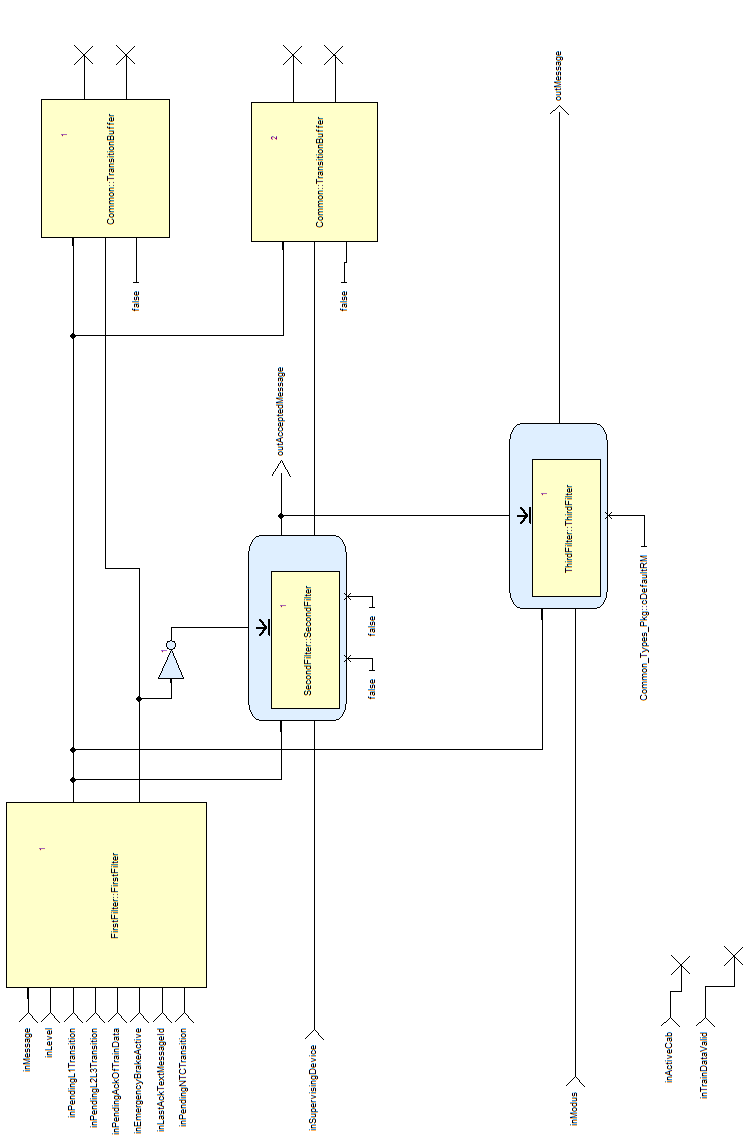
\includegraphics [width=\textwidth]{images/informationfilter-high-level-rot.png}
\caption{High level overview of the InformationFilter components.}
\label{fig:InformationFilterHighLevel}
\end{figure}

\paragraph{Interface}

For an overview of the interface of this internal component we refer to the SCADE model (cf.~link above) respectively the SCADE generated documentation.
